\documentclass[portrait,a0paper,fontscale=0.4]{baposter}

% Packages for input encoding and localization
\usepackage[utf8]{inputenc}
\usepackage[english]{babel}

\usepackage[font=small,labelfont=bf]{caption}
\usepackage{float}
\usepackage{relsize} % http://ftp.gwdg.de/pub/ctan/macros/latex/contrib/relsize/relsize-doc.pdf
\usepackage{tcolorbox}
\usepackage{textcomp}

\definecolor{azure}{rgb}{0.0, 0.5, 1.0}
\definecolor{babyblueeyes}{rgb}{0.63, 0.79, 0.95}
\definecolor{blue-violet}{rgb}{0.54, 0.17, 0.89}
% Package for better URL support
\usepackage{url}

% Package to include graphics
\usepackage{graphicx}
\graphicspath{{./fig/}}
\DeclareGraphicsExtensions{.png,.pdf,.jpg,.jpeg}
\usepackage{subfig}
\usepackage{enumitem}

\setlength{\abovecaptionskip}{-5pt}

\usepackage{palatino}
% Package for program listings
\usepackage{listings}
% Settings for the listings package
\lstset{
  language=C,
  emphstyle={\em},
  }

% Packages for nicer tables
\usepackage{tabularx}
\usepackage{multirow}
\usepackage{booktabs} % for tables
\captionsetup[figure]{labelformat=simple,skip=0.75em,name=Fig.}

\newcommand{\tabularTextSize}[0]{\tiny}
\newcommand{\mycomment}[1]{}
\newcommand{\verytiny}{\fontsize{4}{12} \selectfont \setlength{\baselineskip}{4pt plus 2pt minus 1pt}}
\newcommand{\compresslist}{%
\setlength{\itemsep}{1pt}%
\setlength{\parskip}{0pt}%
\setlength{\parsep}{0pt}%
}


\begin{document}
  \definecolor{UHAM}{HTML}{e30613} %87CEEB
  \definecolor{UHAMLight}{HTML}{e37673} %87CEEB


  % % Setting the watermark image
  % \background
  % {
  %     \begin{tikzpicture}[remember picture,overlay]%
  %     \draw (current page.center) node[opacity=0.3]
  %       {\includegraphics[scale=5]{SIOX-Logo}};
  %     \end{tikzpicture}%
  % }

\begin{poster}
{ % key=value option
  grid=false,
  columns = 4,
  eyecatcher=true,
  background=shadeTB,%user
  bgColorOne=white,
  bgColorTwo=white,
  borderColor=UHAM,
  headerColorOne=UHAMLight,
  headerColorTwo=UHAMLight,%white
  headershape=rounded,
  headerheight=4.8cm,
  textfont={\setlength{\parindent}{0em} \setlength{\parskip}{0.75em}},
  headerborder=open,
  textborder=rounded,
  boxshade=plain,%shadeTB
  boxColorOne=white,
  boxColorTwo=UHAM
}{ % Eye Catcher
  \begin{minipage}{0.2\textwidth}
   \begin{center}
    
\includegraphics[width=0.8\textwidth]{logo-io500.pdf}
   \end{center}
  \end{minipage}

}{ % Poster Title
  \textbf{The Virtual Institute for I/O and the IO-500}
  %\medskip
  %\textbf{\huge xx}
}{ % Poster Authors
  \vspace{0.5em}
  \textsc
  Julian Kunkel$^1$, Jay Lofstead$^2$, John Bent$^3$, George Markomanolis$^4$
  \\[0.5em]
  \emph{$^1$ University of Reading}
  \hspace*{0.25em}
  \emph{$^2$ Sandia National Laboratories}
   \hspace*{0.25em}
  \emph{$^3$ DDN}
  \hspace*{0.25em}
  \emph{$^4$ Oak Ridge National Lab.}
  \\[0.5em]
   Contact: \url{juliankunkel@gmail.com}
}{
    \begin{minipage}{0.2\textwidth}
     \begin{center}
      
\includegraphics[width=0.8\textwidth]{logo-vi4io.png}
     \end{center}
    \end{minipage}
}


\begin{posterbox}[name=problem,column=0]
{Introduction}

The research community in high-performance computing is organized loosely.
There are many distinct resources such as homepages of research groups and benchmarks.
The Virtual Institute for I/O aims to provide a hub for the community and particularly newcomers to find relevant information in many directions.
It hosts the \textbf{comprehensive data center list (CDCL)}. Similarly to the top500, it contains information about supercomputers and their storage systems.

I/O benchmarking, particularly, the intercomparison of measured performance between sites is tricky as there are more hardware components involved and configurations to take into account.
Therefore, together with the community, we standardized an HPC I/O benchmark, the \textbf{IO-500} benchmark, for which the first list had been released during supercomputing in Nov. 2017.
Such a benchmark is also useful to assess the impact of system issues like the \textbf{Meltdown and Spectre* bugs}.

This poster introduces the Virtual Institute for I/O, the high-performance storage list and the effort for the \textbf{IO-500} which are unfunded community projects.
\end{posterbox}


\begin{posterbox}[name=approach,column=0,below=problem]
{The Virtual Institute for I/O}


Goals of the Virtual Institute for I/O (VI4IO) are
\vspace*{-1em}
\begin{itemize}\compresslist
\item Provide a platform for I/O researchers and enthusiasts for exchanging information
\item Foster training and international collaboration in the field of high-performance I/O
\item Track/encourage the deployment of large storage systems by hosting information about high-performance storage systems
\end{itemize}
\vspace*{-1em}

The philosophical cornerstones of VI4IO are:

\vspace*{-1em}
\begin{itemize}\compresslist
\item Treat contributors/participants equally
\item Allow free participation without any fee inclusive to all
\item Independent of vendors/research facilities
\end{itemize}
\end{posterbox}


\begin{posterbox}[name=overview,column=0,below=approach]{Open Organization}

The organization uses a wiki as central hub
\vspace*{-1em}
\begin{itemize}\compresslist
\item Registered users can edit the content
\item Mayor changes should be discussed on the contribute mailing list
\item Tag clouds link between similar entities
\item Supported by mailing lists, e.g.:
\begin{itemize}\compresslist
\item Call-for-papers
\item Announcements
\item Contributions / suggestions
\end{itemize}
\end{itemize}

\end{posterbox}


\begin{posterbox}[name=wps,column=0,below=overview, above=bottom]{Community Content}
The wiki covers \textbf{A) worldwide research groups that address high-performance I/O including:}

\vspace*{-1em}
\begin{itemize}\compresslist
\item A taglist for available knowledge
\item Research products such as file systems
\item Ongoing research projects
\end{itemize}

\vspace*{-0.5em}

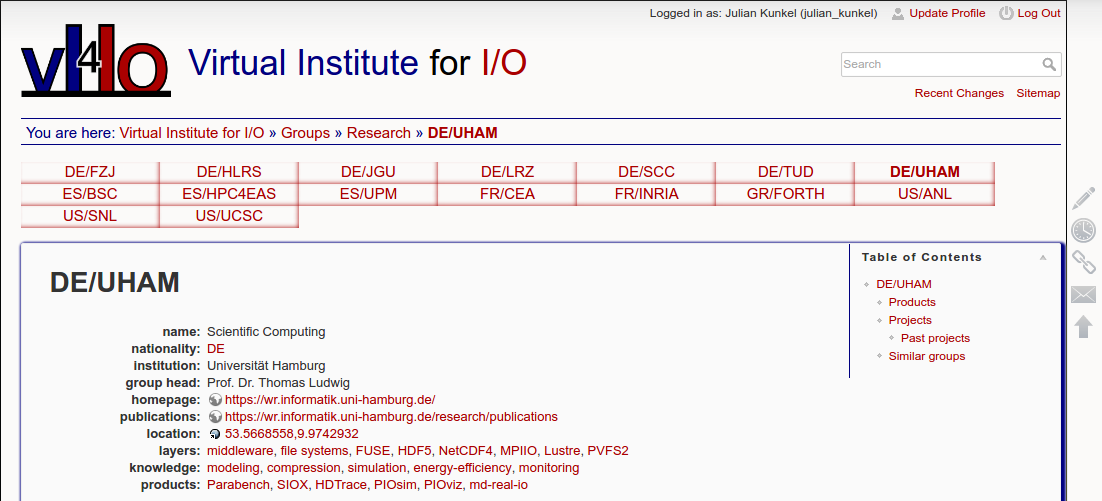
\includegraphics[width=7.5cm]{groups}

Everyone is welcome to add (own) group(s)!

\textbf{B) Relevant I/O related tools and benchmarks}

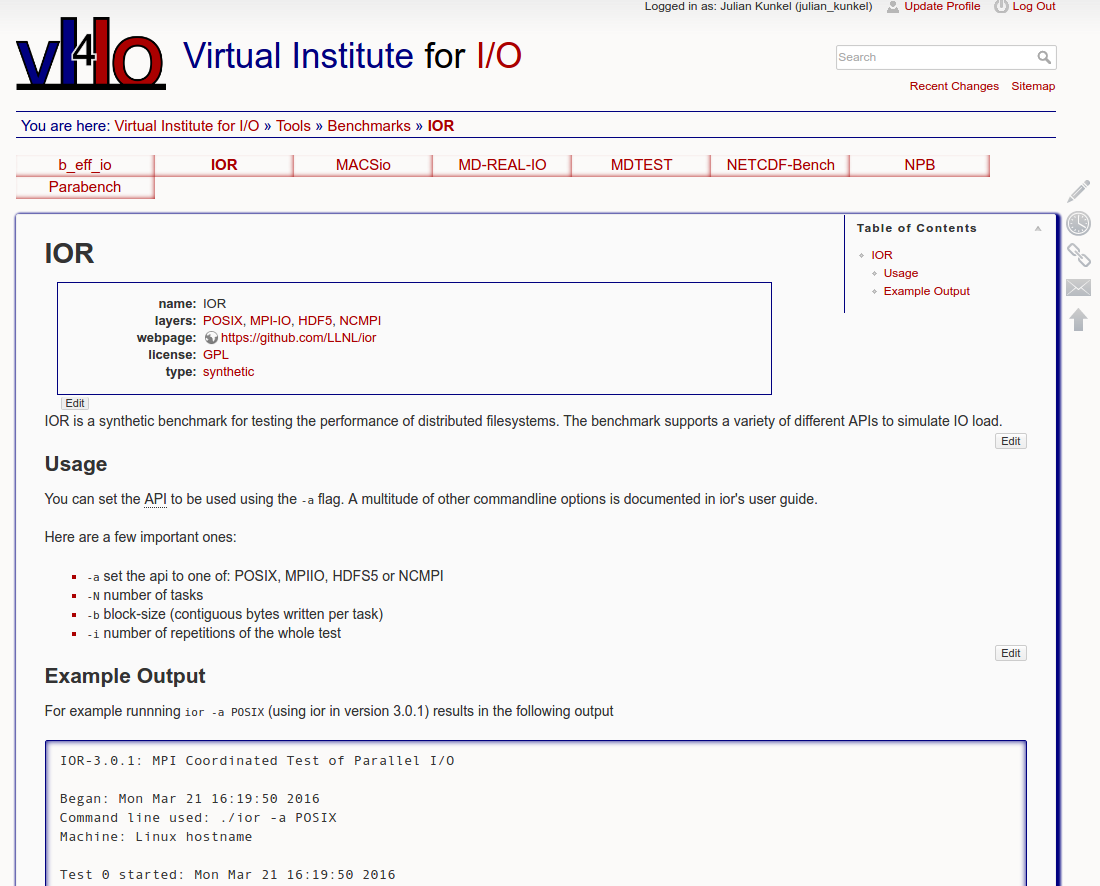
\includegraphics[width=7cm]{benchmark}


\textbf{C) Comprehensive Data Center List} \\ (see the other boxes)

\medskip

\end{posterbox}


%%%%%%%%%%%%%%%%%%%%%%%%%%%%%%%%%%%%%%%%%%%%%%%%%%%%%%%
\begin{posterbox}[name=io500,column=1,span=2]{IO-500 Effort}
Together with the community, we created the IO-500 benchmark to compare storage systems.

\textbf{Goals for the benchmark:}

\vspace*{-2em}
\begin{minipage}{10.5cm}
\begin{itemize} \compresslist
\item Capture user-experienced performance % and honor system balance
\item Reported performance is representative for:
%\vspace*{-0.5em}
\begin{itemize} \compresslist
\item IOEasy: Applications with well optimized I/O patterns
\item IOHard: Applications that require a random workload
\item MDEasy: Metadata/small objects
\item MDHard: Small files (3901 bytes) in a shared directory
\item Find: Finding relevant objects based on patterns
\end{itemize}
\end{itemize}
\end{minipage}
\qquad
\begin{minipage}{4cm}
  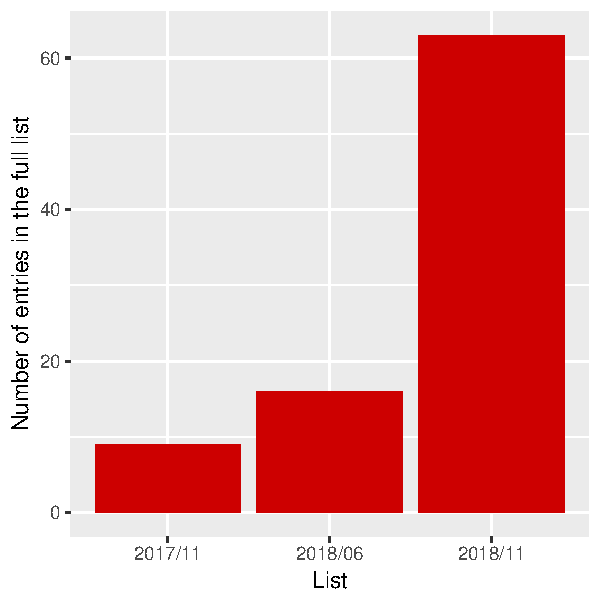
\includegraphics[width=3.8cm]{io-500-history.pdf}
  \captionof{figure}{Growth of the list}
\end{minipage}
%\qquad
%\begin{minipage}{6cm}
%x
%\end{minipage}

\vspace*{-1.5em}


\textbf{Challenges:}
\vspace*{-1em}
\begin{itemize} \compresslist
\item Representative: for optimized, naive I/O heavy workloads; and small objects
\item Inclusive: cover various storage technology and non-POSIX APIs
\item Trustworthy: representative results and prevent cheating
\item Cheap: easy to run and short benchmarking time (in the order of minutes)
\end{itemize}

\vspace*{-1em}

\textbf{Benefit for the community beyond the IO-500:}
\vspace*{-1em}
\begin{itemize} \compresslist
\item Support the development of benchmarks that are used (IO-500 builds on standard benchmarks)
\item Feed back best practices of tool usage (e.g., find) and benchmarks
\item Aid detailed comparison of individual system characteristics while having a \textbf{ranked list}
\item Share best-practices to obtain good performance
\end{itemize}


\end{posterbox}


\begin{posterbox}[name=io500res,column=1,above=bottom,below=io500]{IO-500 List Nov 2018}

There are several lists available, the \textbf{full list} contains all the results submitted for comparison while entries can enter a \textbf{ranked list} upon user choice and only one solution per system.

There are several ranked lists with awards that stimulate aspects of I/O system development:
\vspace*{-0.75em}
\begin{itemize}\compresslist
  \item The \textit{IO-500 award} for the fastest system in the ranked IO-500 list
  \item The \textit{10 node challenge} fosters performance for small-scale runs
\end{itemize}
\vspace*{-1em}
Further awards may follow.

\textbf{The ranked IO-500 list:}

%
\includegraphics[width=\textwidth]{logo-io500.pdf}
%\vspace*{1em}
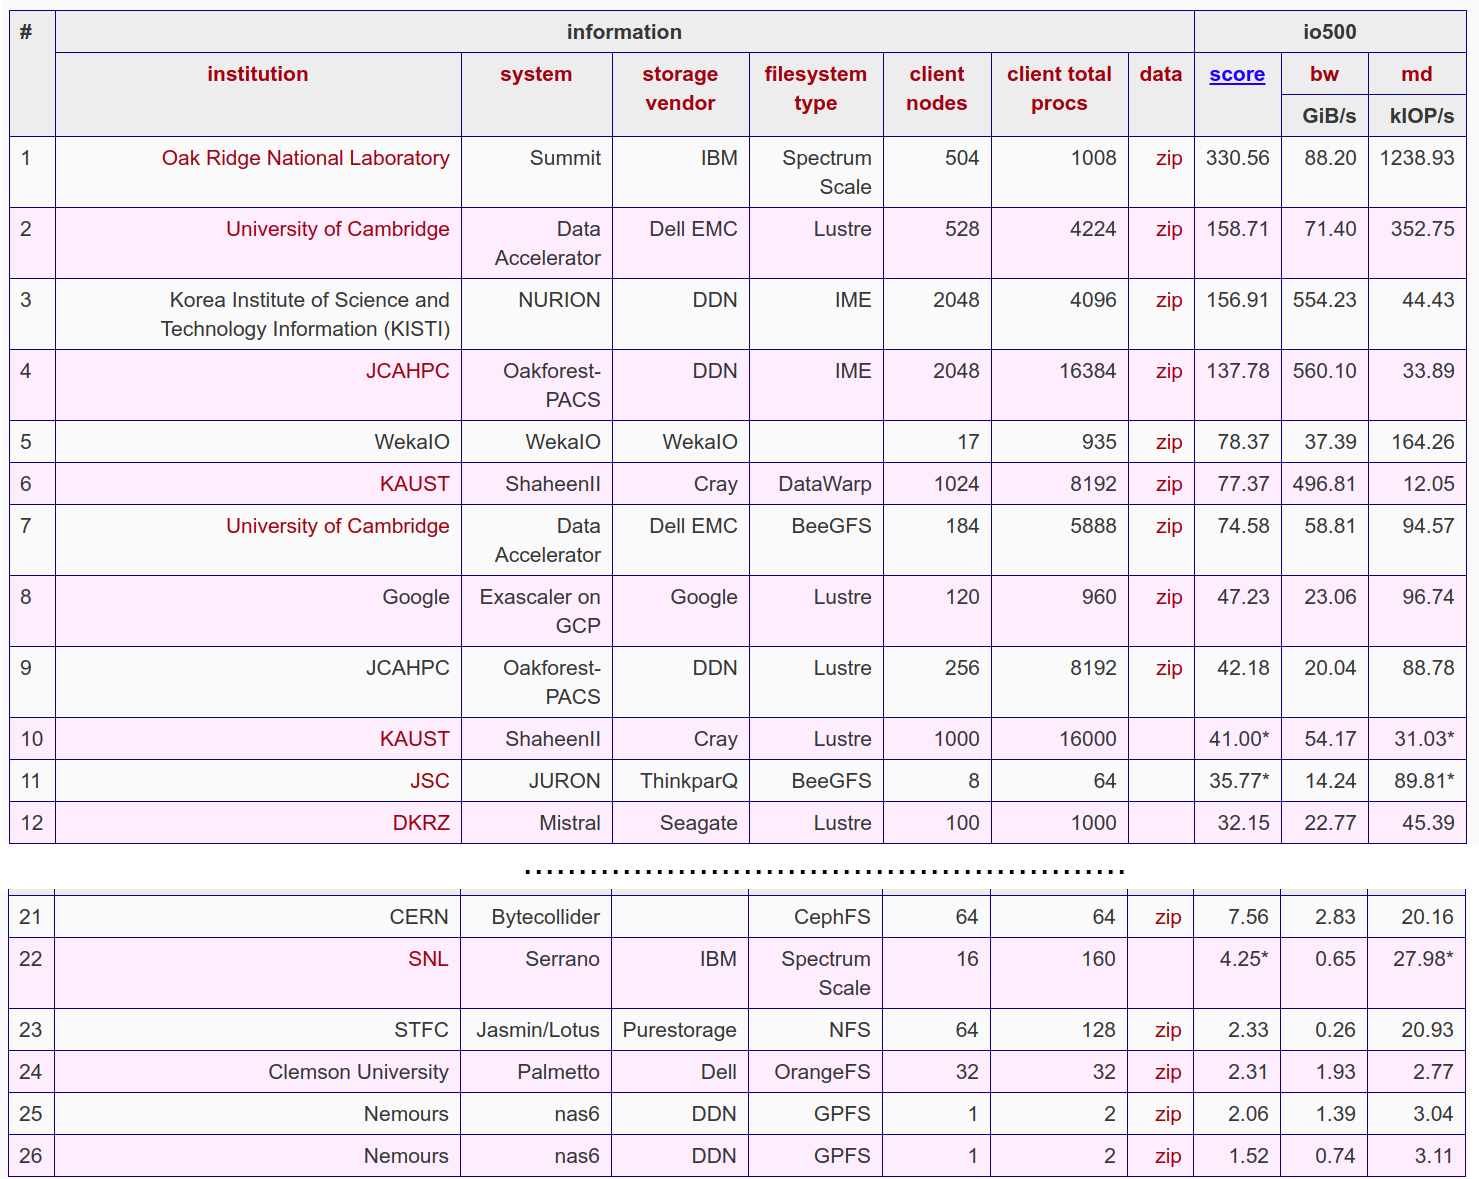
\includegraphics[width=\textwidth]{io500}


\vspace*{-1em}


\paragraph{Flexible equations}

It supports equations to compute derived metrics, here \textit{mdtest.easy\_write / client\_nodes} for the full list:

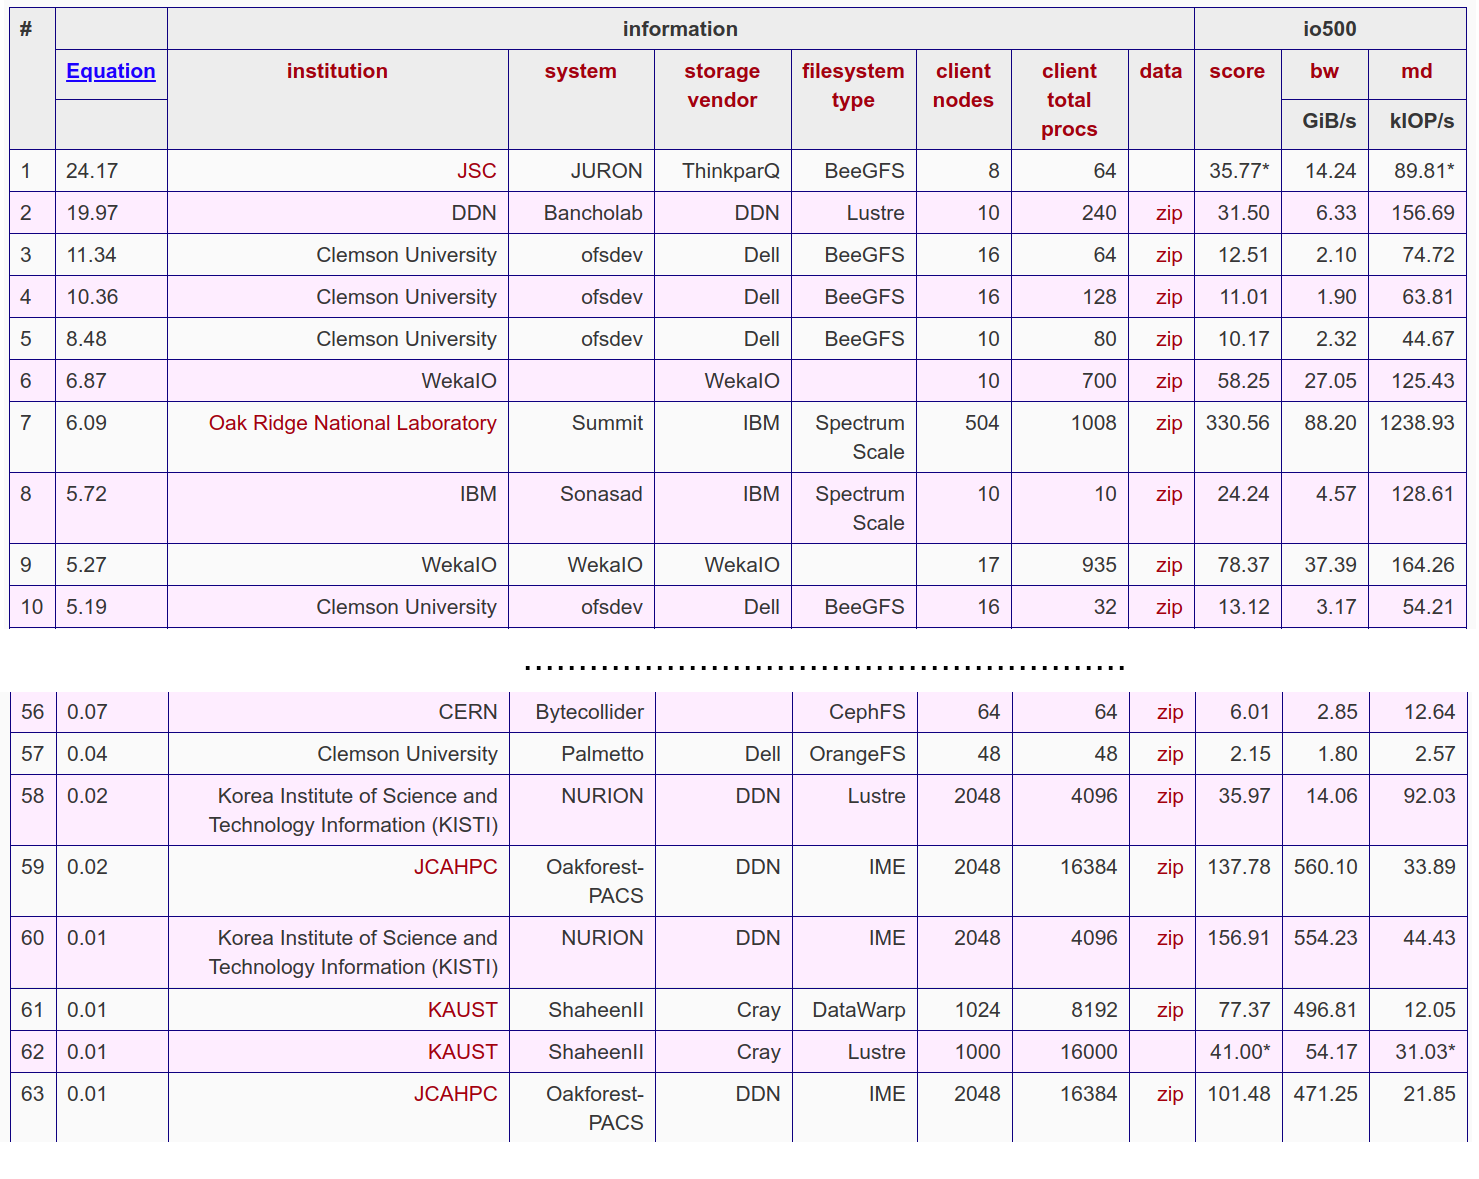
\includegraphics[width=\textwidth]{io500-sorted}

The system displays a net graph for further distinguishing the best systems:

\vspace*{-1.5em}

\begin{center}
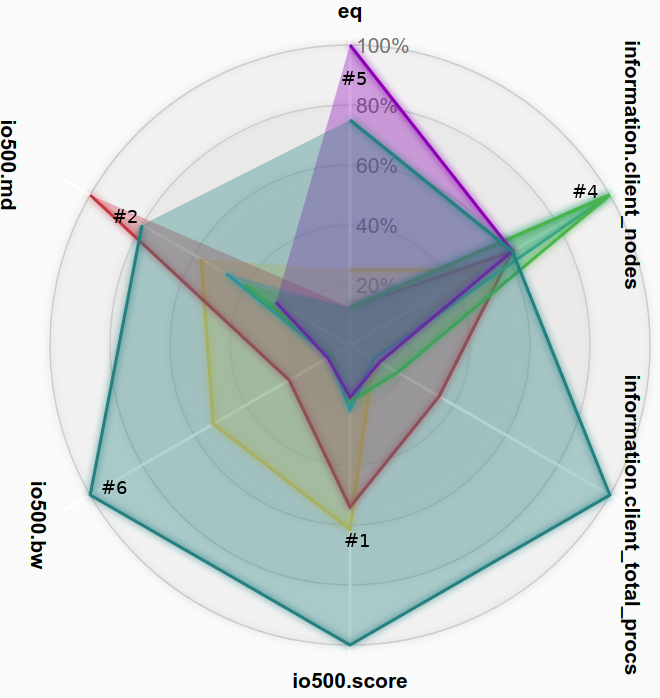
\includegraphics[width=0.6\textwidth]{io-500-net}
\end{center}

\vspace*{-1.5em}

As we can see, this can be used to create arbitrary new rankings and investigate the data.

\vspace*{-1em}

\paragraph{All results are available}

The individual submission scripts and results for the benchmarks are preserved and can be accessed.
The data is also available as CSV file for offline analysis.


%This feature will be extended to support data from the CDCL.
\end{posterbox}



\begin{posterbox}[name=schedule,column=2,span=1, above=bottom, below=io500]{Data Center List}
The comprehensive data center list with its system model describes how characteristics are assigned to components.
Storage is difficulty to assign to a single component as it is often shared across supercomputers,
therefore, a flexible component based model is used.

Supported components:
\vspace*{-1em}
\begin{itemize}\compresslist
\item Site: Describes the facility
\item Supercomputer: A system
\item Storage system
\item Nodes
\item Network
\item Building
\end{itemize}

\vspace*{-1em}

The schema is under active development -- we aim to describe data center characteristics.
The web page allows the creation of a topology for the facility to indicate the relation between the components -- ultimately multiple views will be created to show, e.g.:

\vspace*{-1em}

\begin{itemize} \compresslist
  \item Logical network connectivity
  \item Physical layout in racks
  \item Building organization
\end{itemize}

\vspace*{-1em}


\textbf{Metrics:} Most metrics can be determined without measurement and describe hardware and software characteristics that should be known to the site and vendor. A few metrics cover actually observed metadata and I/O performance, in this case the measurement procedure must be defined.
The list stores data entered in the wiki into a database and converts data to a base unit.

The following is an example of the schema for the DKRZ system:

\vspace*{-0.65em}

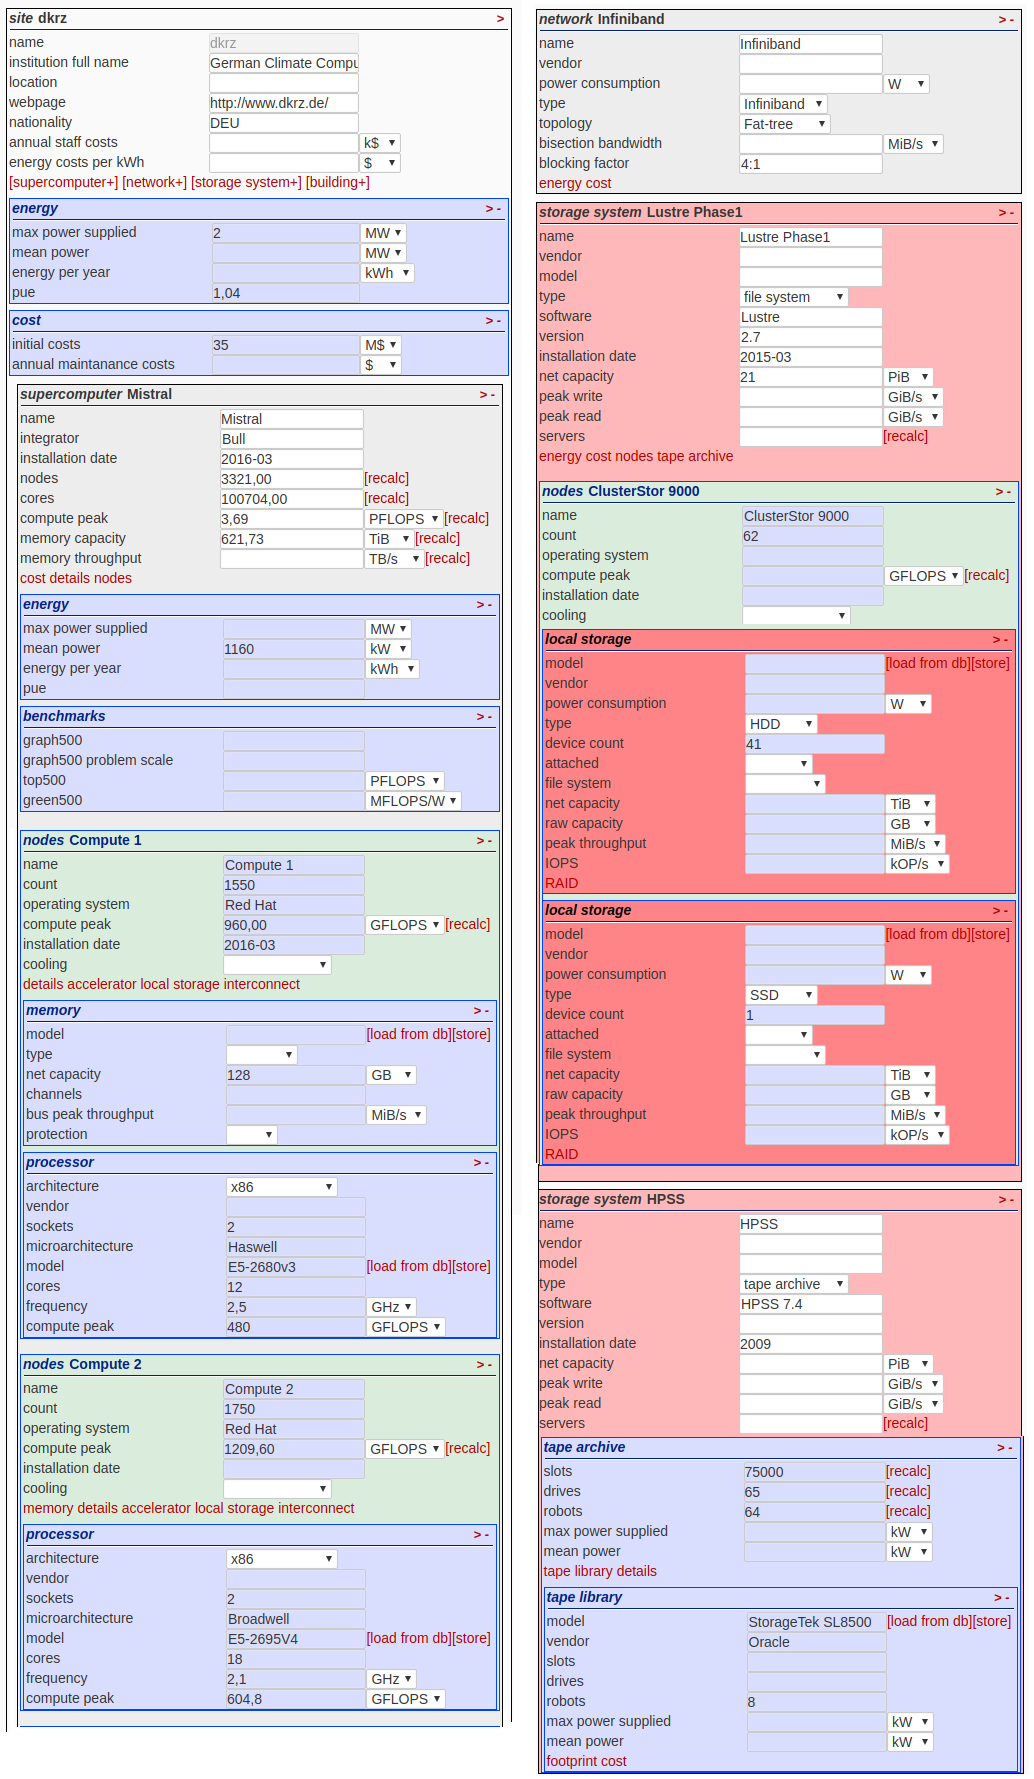
\includegraphics[width=\textwidth]{schema}

\vspace*{-1em}

The rules for determining performance are relaxed due to the complexity of I/O measurements, but this is augmented by the IO-500.
\end{posterbox}

%%%%%%%%%%%%%%%%%%%%%%%%%%%%%%%%%%%%%%%%%%%%%%%%%%%%%%%



\begin{posterbox}[name=engineering,column=3]{HPSL 2019}
The current list contains 43 sites:

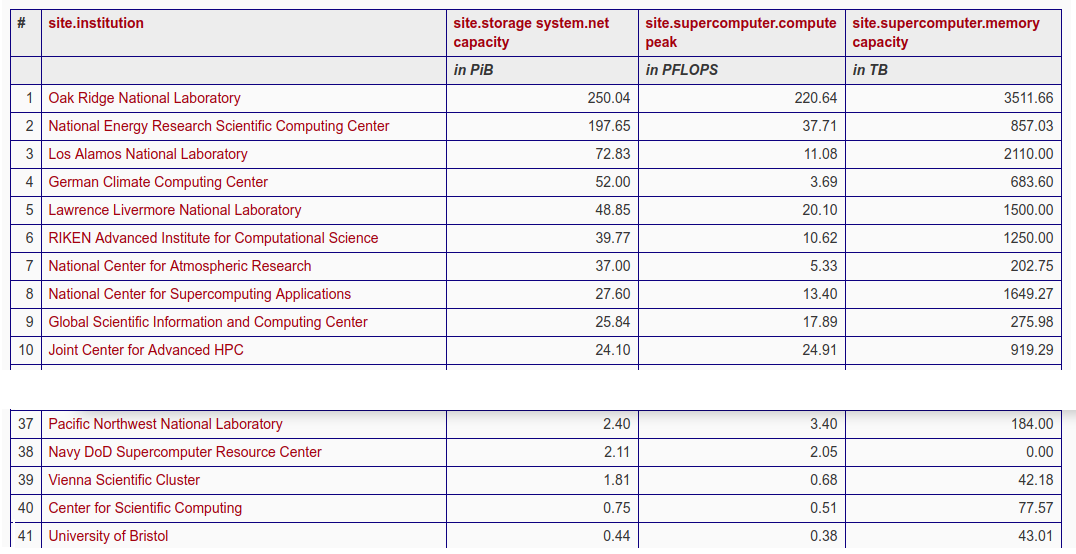
\includegraphics[width=\textwidth]{dcl-2018}

Various views are possible, moreover, it
supports flexible data aggregation, e.g., capacity by country:

\vspace*{-2em}

\begin{center}
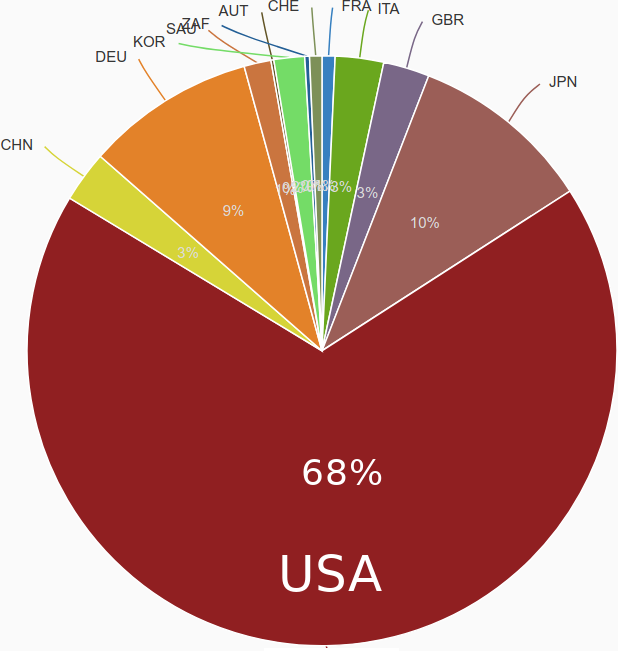
\includegraphics[width=0.6\textwidth]{aggregated-by-country}
\end{center}

\vspace*{-1em}

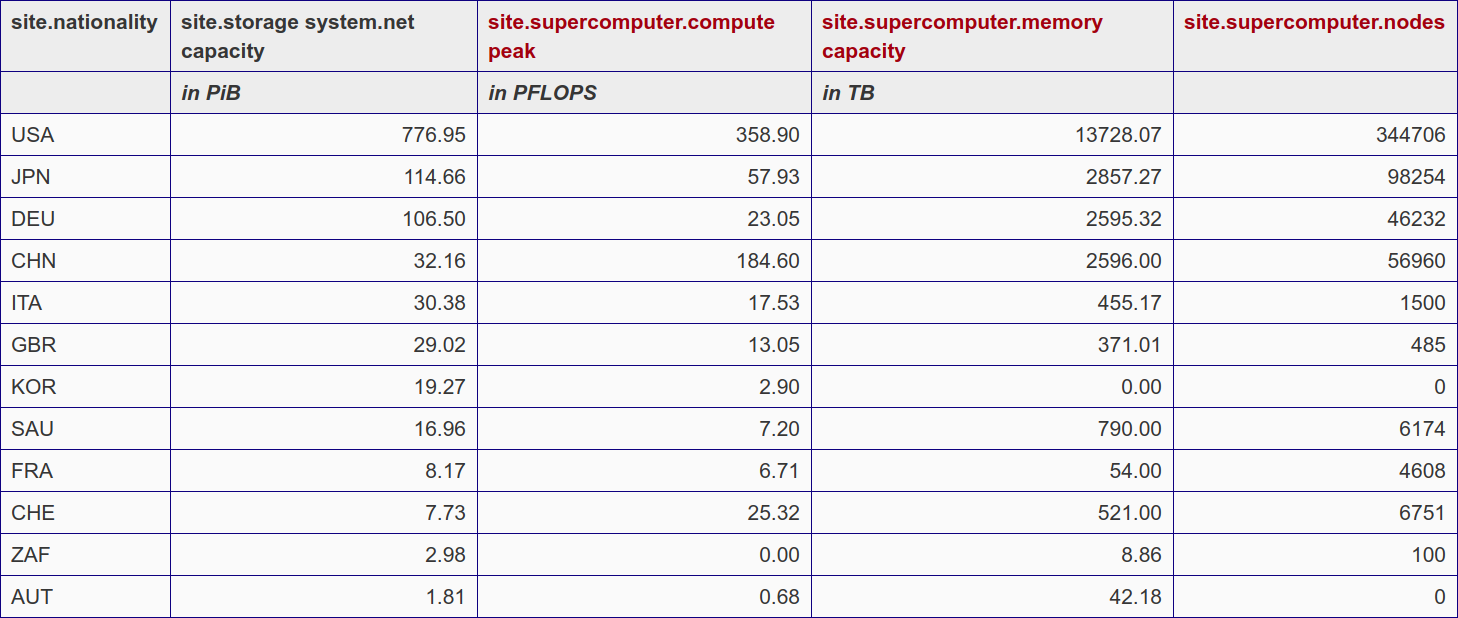
\includegraphics[width=\textwidth]{capacity-grouped}

\end{posterbox}




\begin{posterbox}[name=awareness,column=3,below=engineering]{Derived Analysis}
With the collected data many in-depth analysis becomes possible, for example,
the relationship between storage and memory capacity:

\vspace*{-1em}

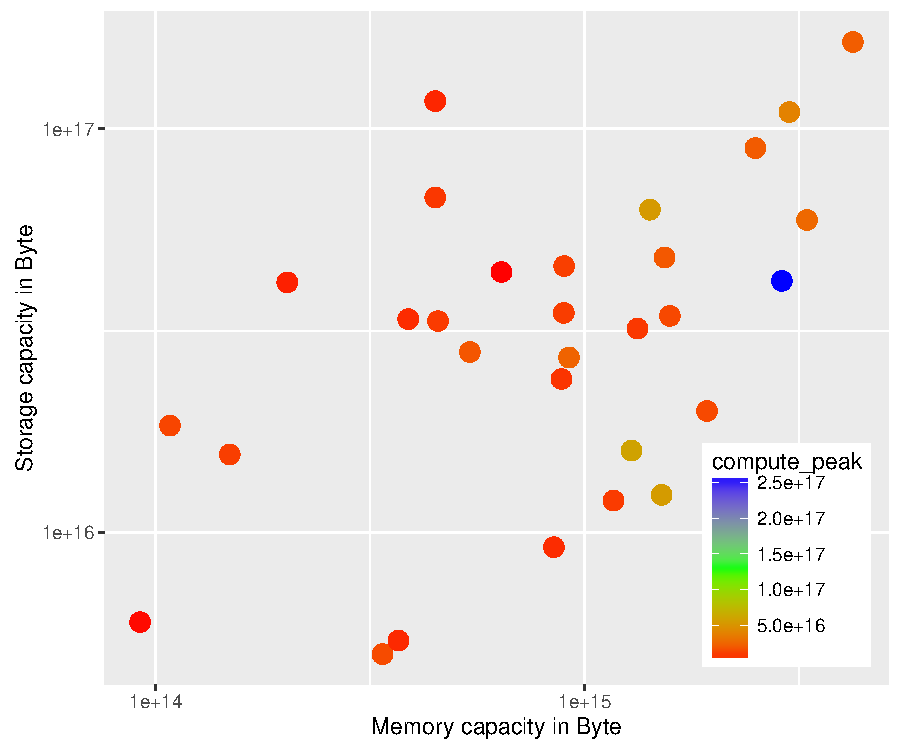
\includegraphics[width=5cm]{memstorage}
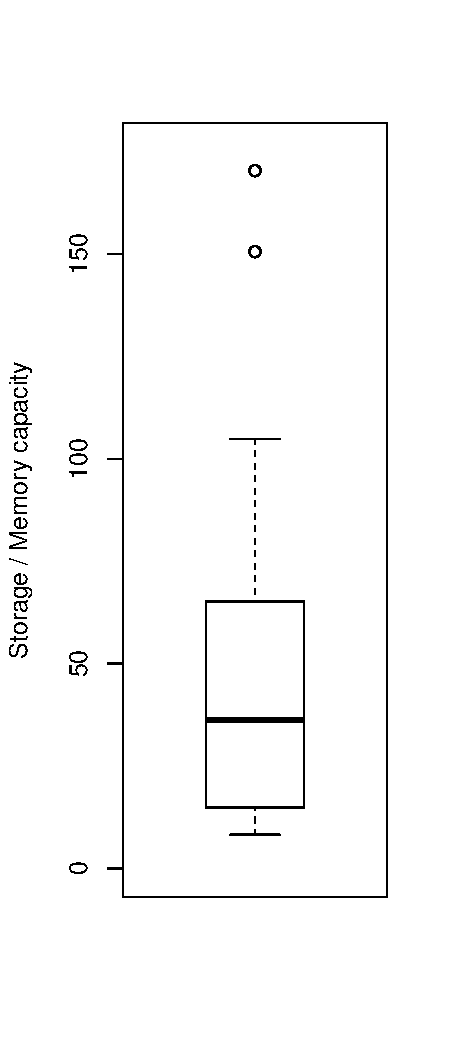
\includegraphics[width=2cm]{capacitymemory}

\vspace*{-2em}
\begin{itemize}\compresslist
\item Correlation storage capacity vs.
  \begin{itemize}\compresslist
  \item memory capacity = 0.63
  \item compute peak = 0.057
  \end{itemize}
\item Mean(storage/mem capacity) = 58
\end{itemize}

\end{posterbox}

\begin{posterbox}[name=b4,column=3,below=awareness]{Ongoing Work}
\begin{itemize}\compresslist
\item IO-500:
  \begin{itemize}
  \item Clarified execution rules
  \item Procedures to adapt IO-500
  \item Integration of optional benchmarks
  \item Continuous integration deployment \\
        Including performance regression
  \item Finalize vendor engagement program
  \end{itemize}
\item VI4IO standardization efforts
  \begin{itemize}\compresslist
  \item Data center representation
  \item Next-generation interfaces (NGI)
  \end{itemize}
\item CDCL list
  \begin{itemize}\compresslist
  \item Extended schema and alternative views
  \item More CDCL sites
  \item Better link between IO-500 and CDCL
  \end{itemize}
\item Support training and teaching for storage
\end{itemize}
\end{posterbox}


\begin{posterbox}[name=hpccertification,column=3,below=b4, above=bottom]{VI4IO, IO-500, and You}


%\begin{minipage}{0.7\textwidth}
You are welcome to join the mailing lists or our slack channel and participate!


\begin{minipage}{0.7\textwidth}
\Large Join us on Slack:
\end{minipage}
\begin{minipage}{0.29\textwidth}

\includegraphics[width=\textwidth]{qr-join-slack-com.pdf}
\end{minipage}

The content is under open licenses.
%\end{minipage}
%\begin{minipage}{0.29\textwidth}
%
\includegraphics[width=\textwidth]{qr-code.jpg}
%\end{minipage}


More details on:

\vspace*{-1.5em}

\begin{itemize}
  \compresslist
  \Large
  \item \url{https://vi4io.org}
  \item \url{http://io-500.org}
\end{itemize}



\end{posterbox}


\end{poster}
\end{document}
